\documentclass[aspectratio=169]{beamer}
\usepackage{color,amsmath}
\usepackage{subfigure}
\usepackage{booktabs}
\usepackage{framed}
\usepackage{comment}


%%%%%%%%%%%%%%%%%%%%%%%%%%
\title[]{Moving beyond simple experiments}
\author[]{Matthew J. Salganik\\Department of Sociology\\Princeton University}
\date[]{Summer Institutes in Computational Social Science\\June 22, 2019
\vfill
\begin{flushleft}
{\scriptsize
The Summer Institutes in Computational Social Science is supported by grants from the Russell Sage Foundation and the Alfred P. Sloan Foundation.}
\end{flushleft}
\begin{flushright}

\includegraphics[width=0.1\textwidth]{figures/cc-by.png}
\end{flushright}
}
\begin{document}
%%%%%%%%%%%%%%%%%%%%%%%%%%
\frame{\titlepage}
%%%%%%%%%%%%%%%%%%%%%%%%%%
\begin{frame}

\Large{
\begin{center}
Optimization experiments vs  Understanding experiments
\end{center}
}

\end{frame}
%%%%%%%%%%%%%%%%%%%%%%%
\begin{frame}

\Large{
\begin{center}
Optimization experiments + Understanding experiments
\end{center}
}

\end{frame}
%%%%%%%%%%%%%%%%%%%%%%%
\begin{frame}

\begin{figure}
  \centering
  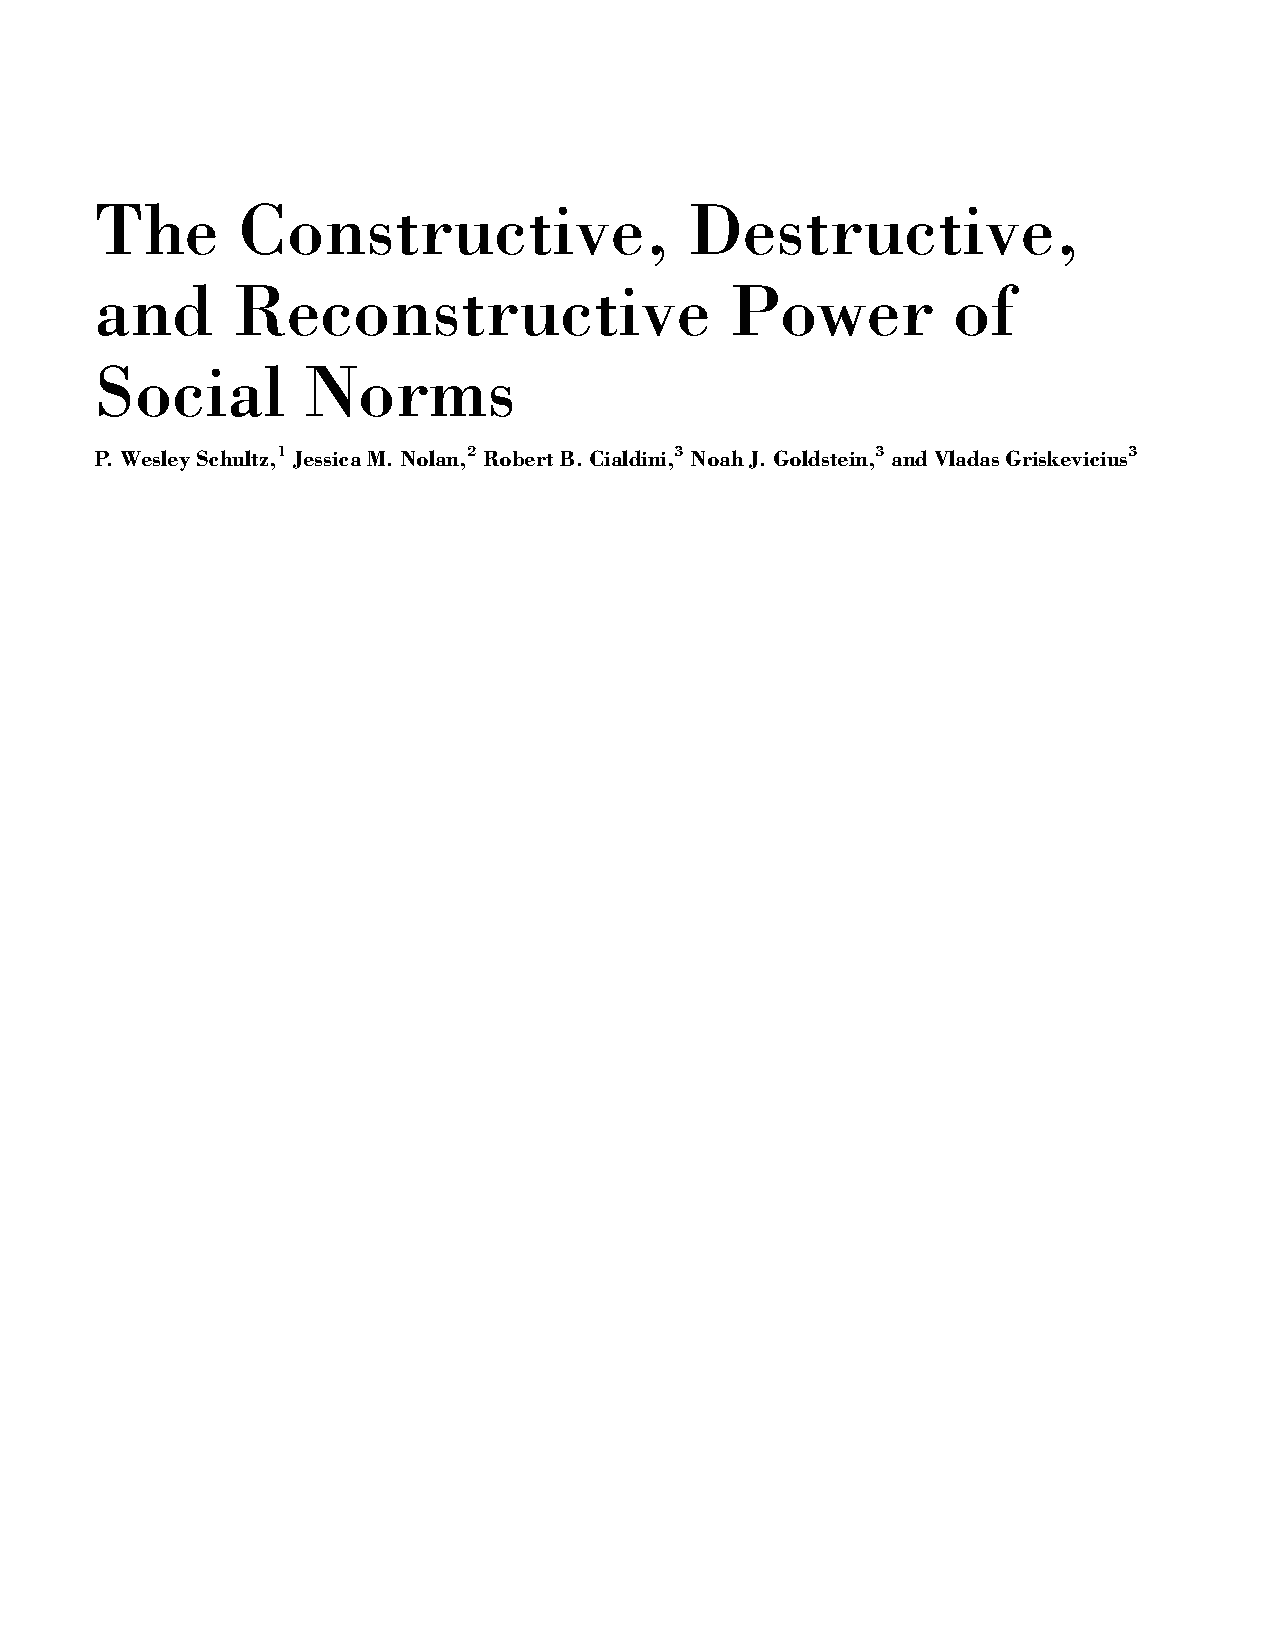
\includegraphics[width = 0.9\textwidth]{figures/schultz_constructive_2007_title}
\end{figure}

\vfill
\tiny{\url{http://dx.doi.org/10.1111/j.1467-9280.2007.01917.x}}

\end{frame}
%%%%%%%%%%%%%%%%%%%%%%%
\begin{frame}

\begin{figure}
  \centering
  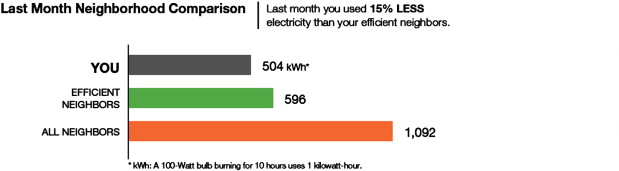
\includegraphics[width = \textwidth]{figures/energy_peers_no_emoticon}
\end{figure}

\vfill
\tiny{Figures from Allcott (2011)}

\end{frame}
%%%%%%%%%%%%%%%%%%%%%%%%
\begin{frame}

\begin{figure}
  \centering
  \only<1>{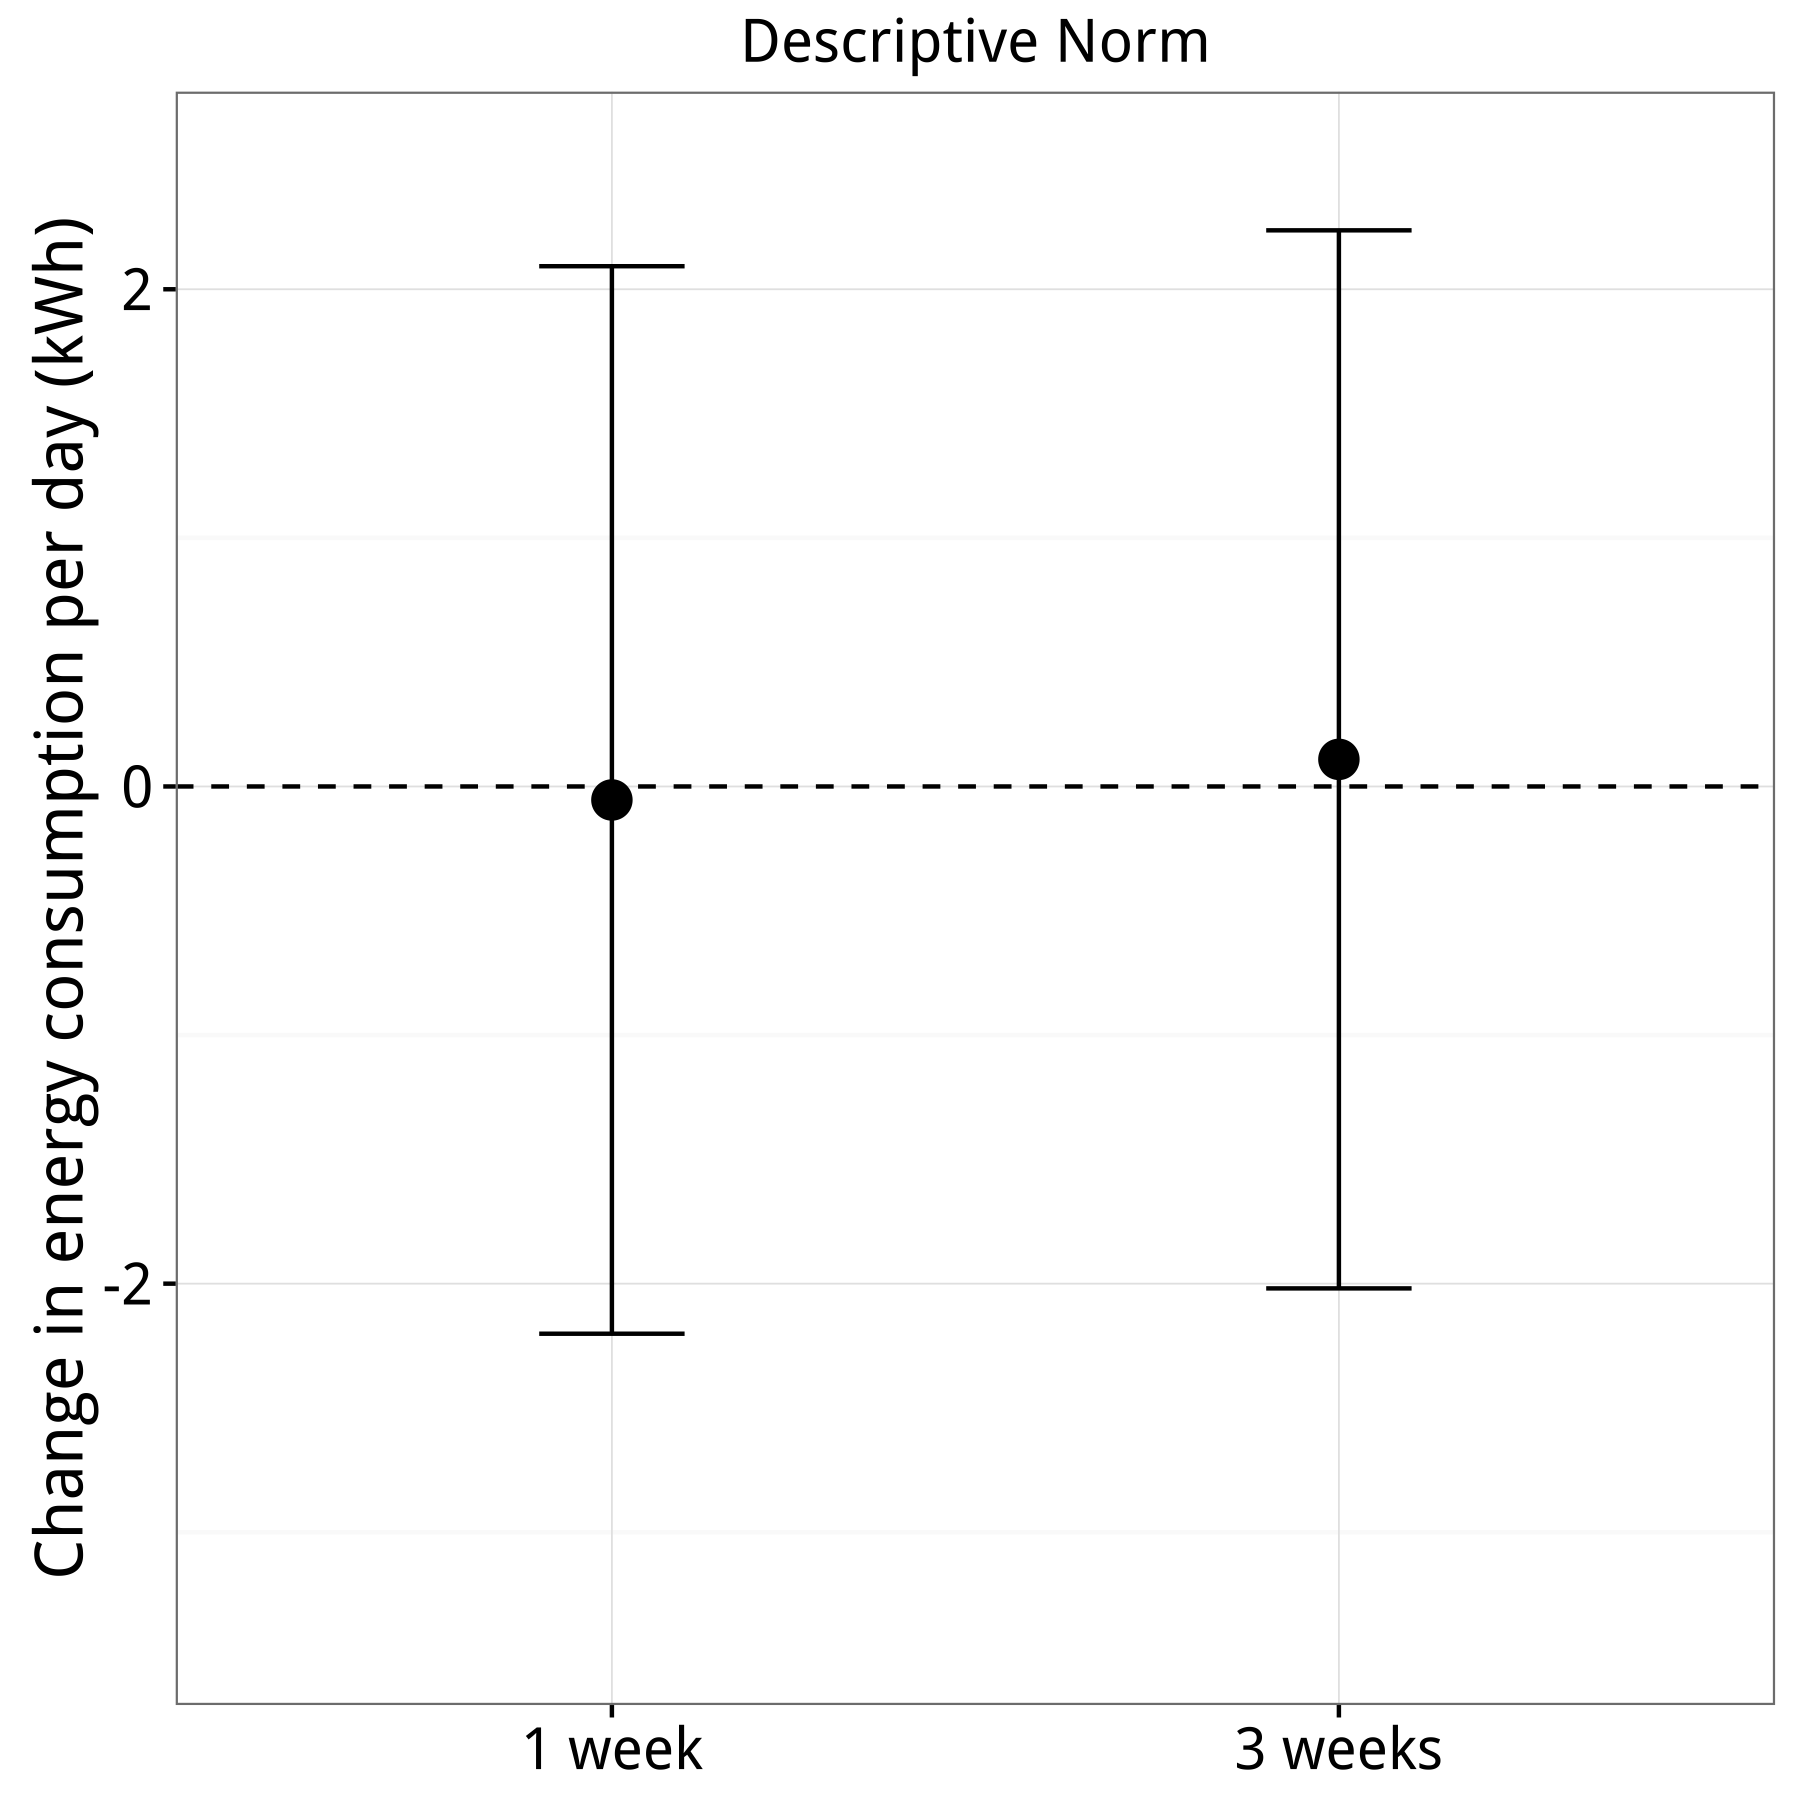
\includegraphics[width = 0.5\textwidth]{figures/schultz_constructive_2007_1panel}}
  \only<2>{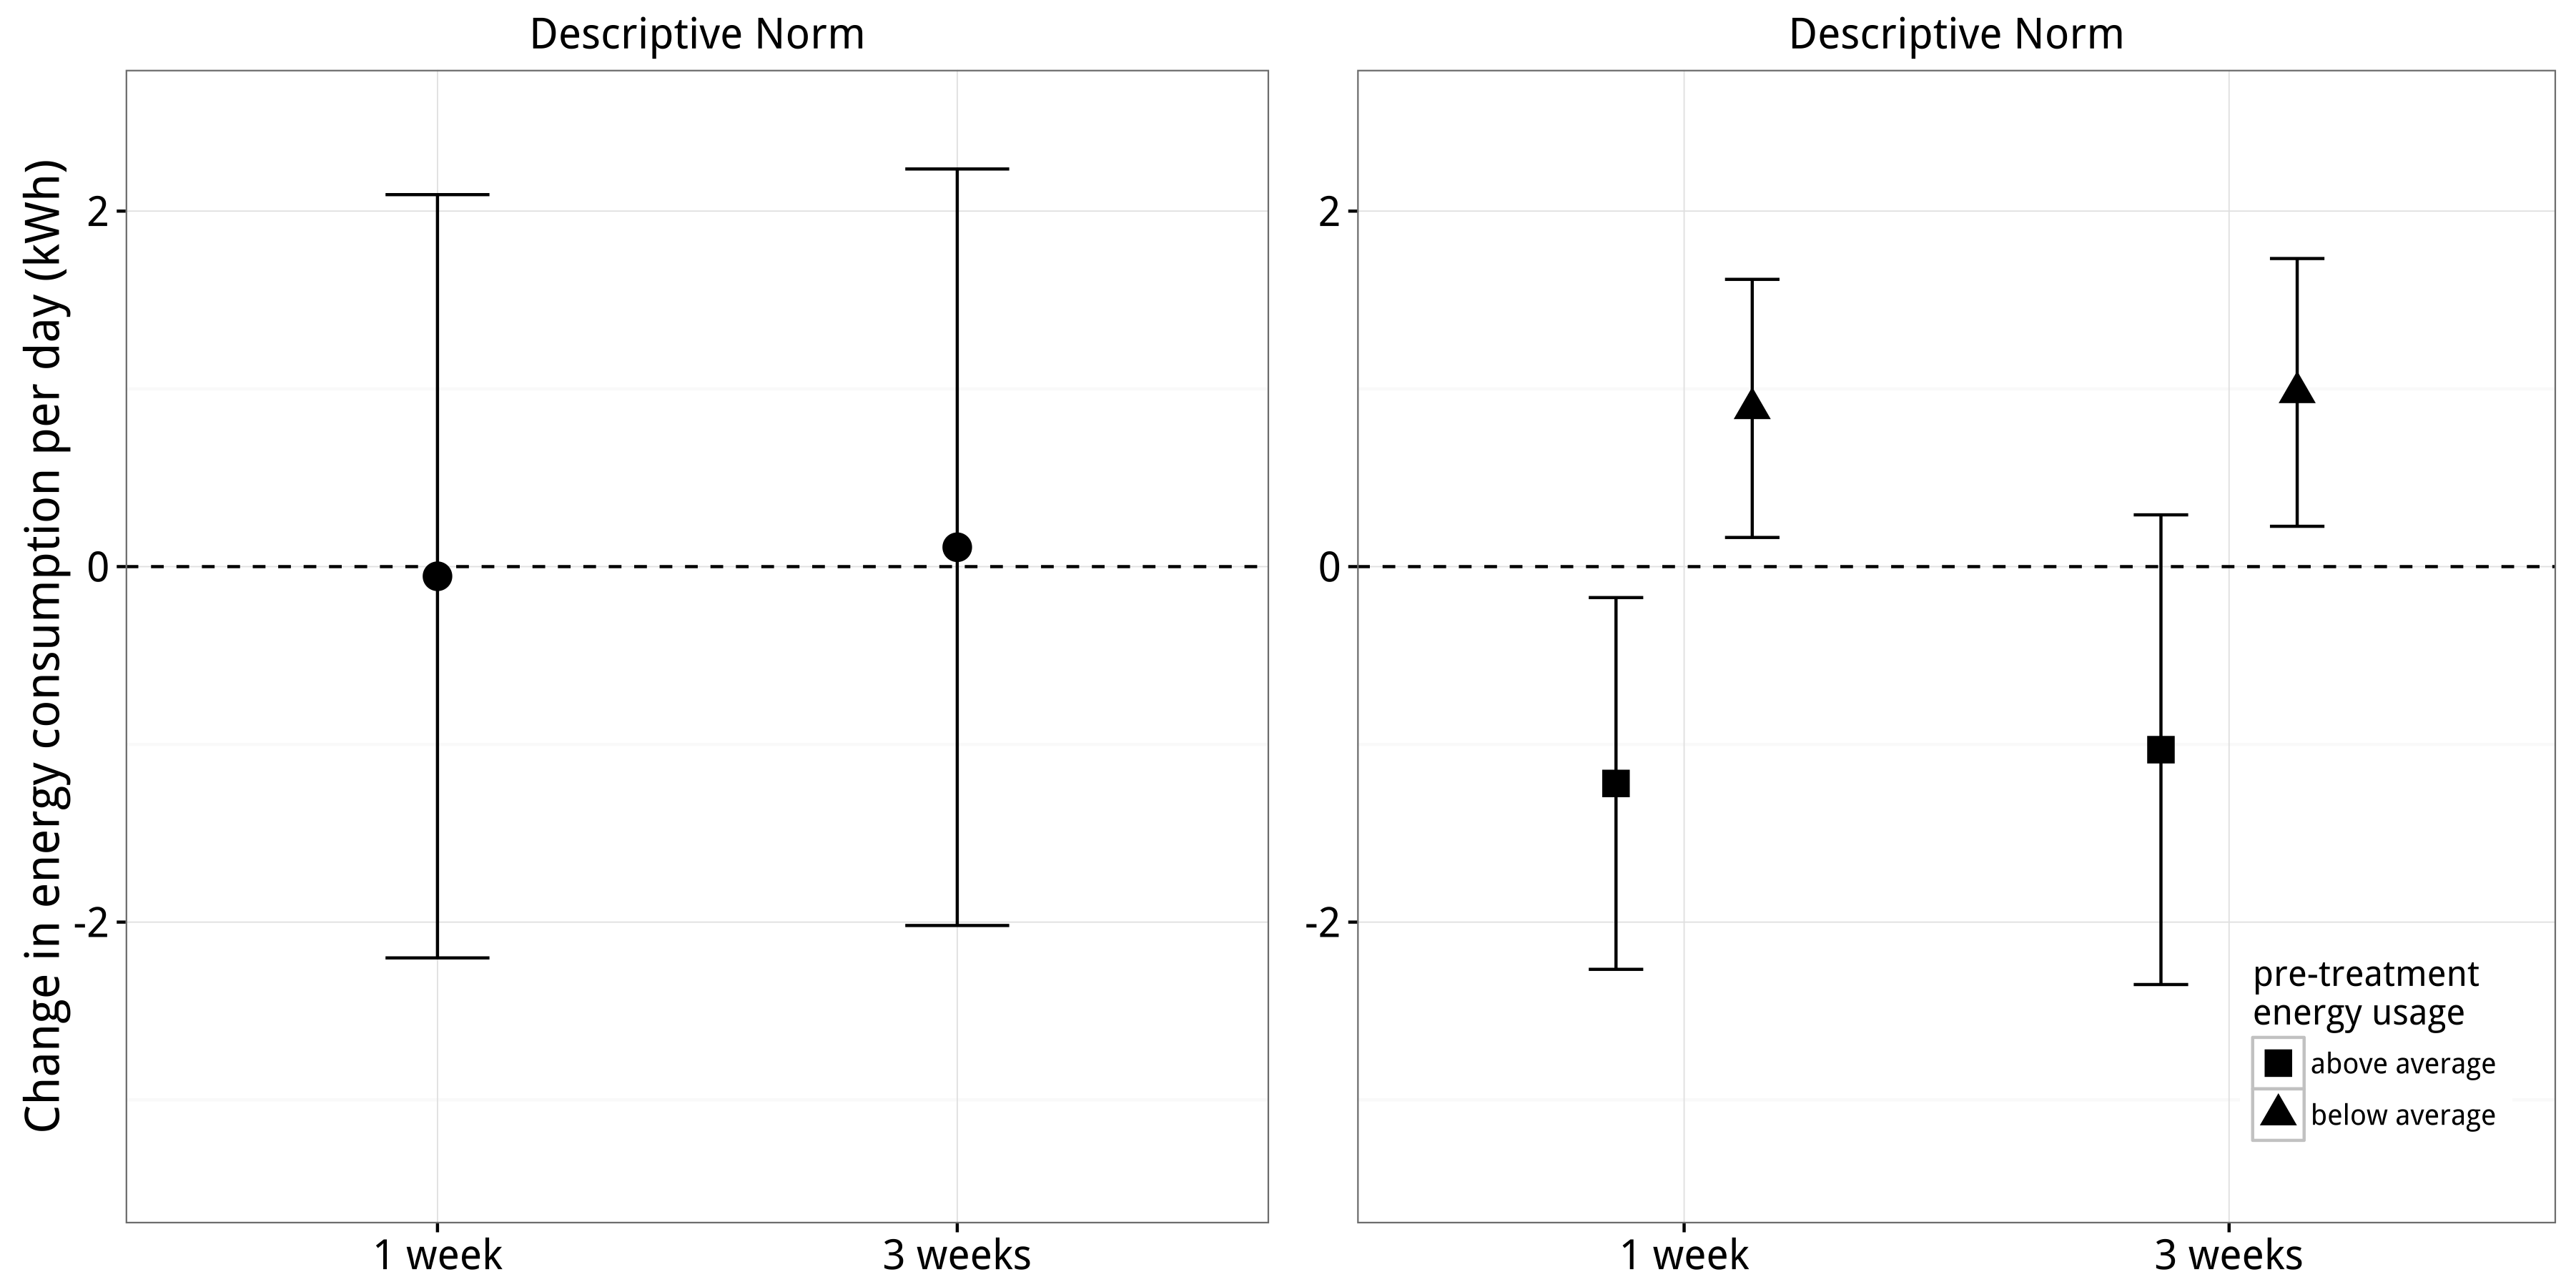
\includegraphics[width = 0.8\textwidth]{figures/schultz_constructive_2007_2panel}}
\end{figure}

\end{frame}
%%%%%%%%%%%%%%%%%%%%%%%%
\begin{frame}

\begin{figure}
  \centering
  \only<1>{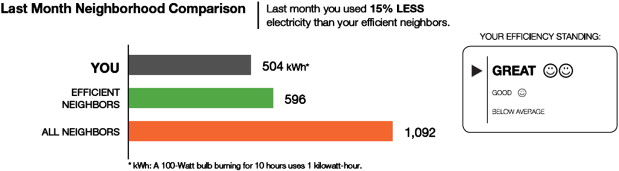
\includegraphics[width = \textwidth]{figures/allcott_social_2011_fig1}}
  \only<2>{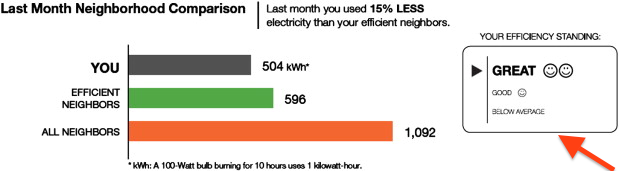
\includegraphics[width = \textwidth]{figures/allcott_social_2011_fig1_arrow}}
\end{figure}

\vfill
\tiny{Figures from Allcott (2011)}

\end{frame}
%%%%%%%%%%%%%%%%%%%%%%%%
\begin{frame}

\begin{figure}
  \centering
  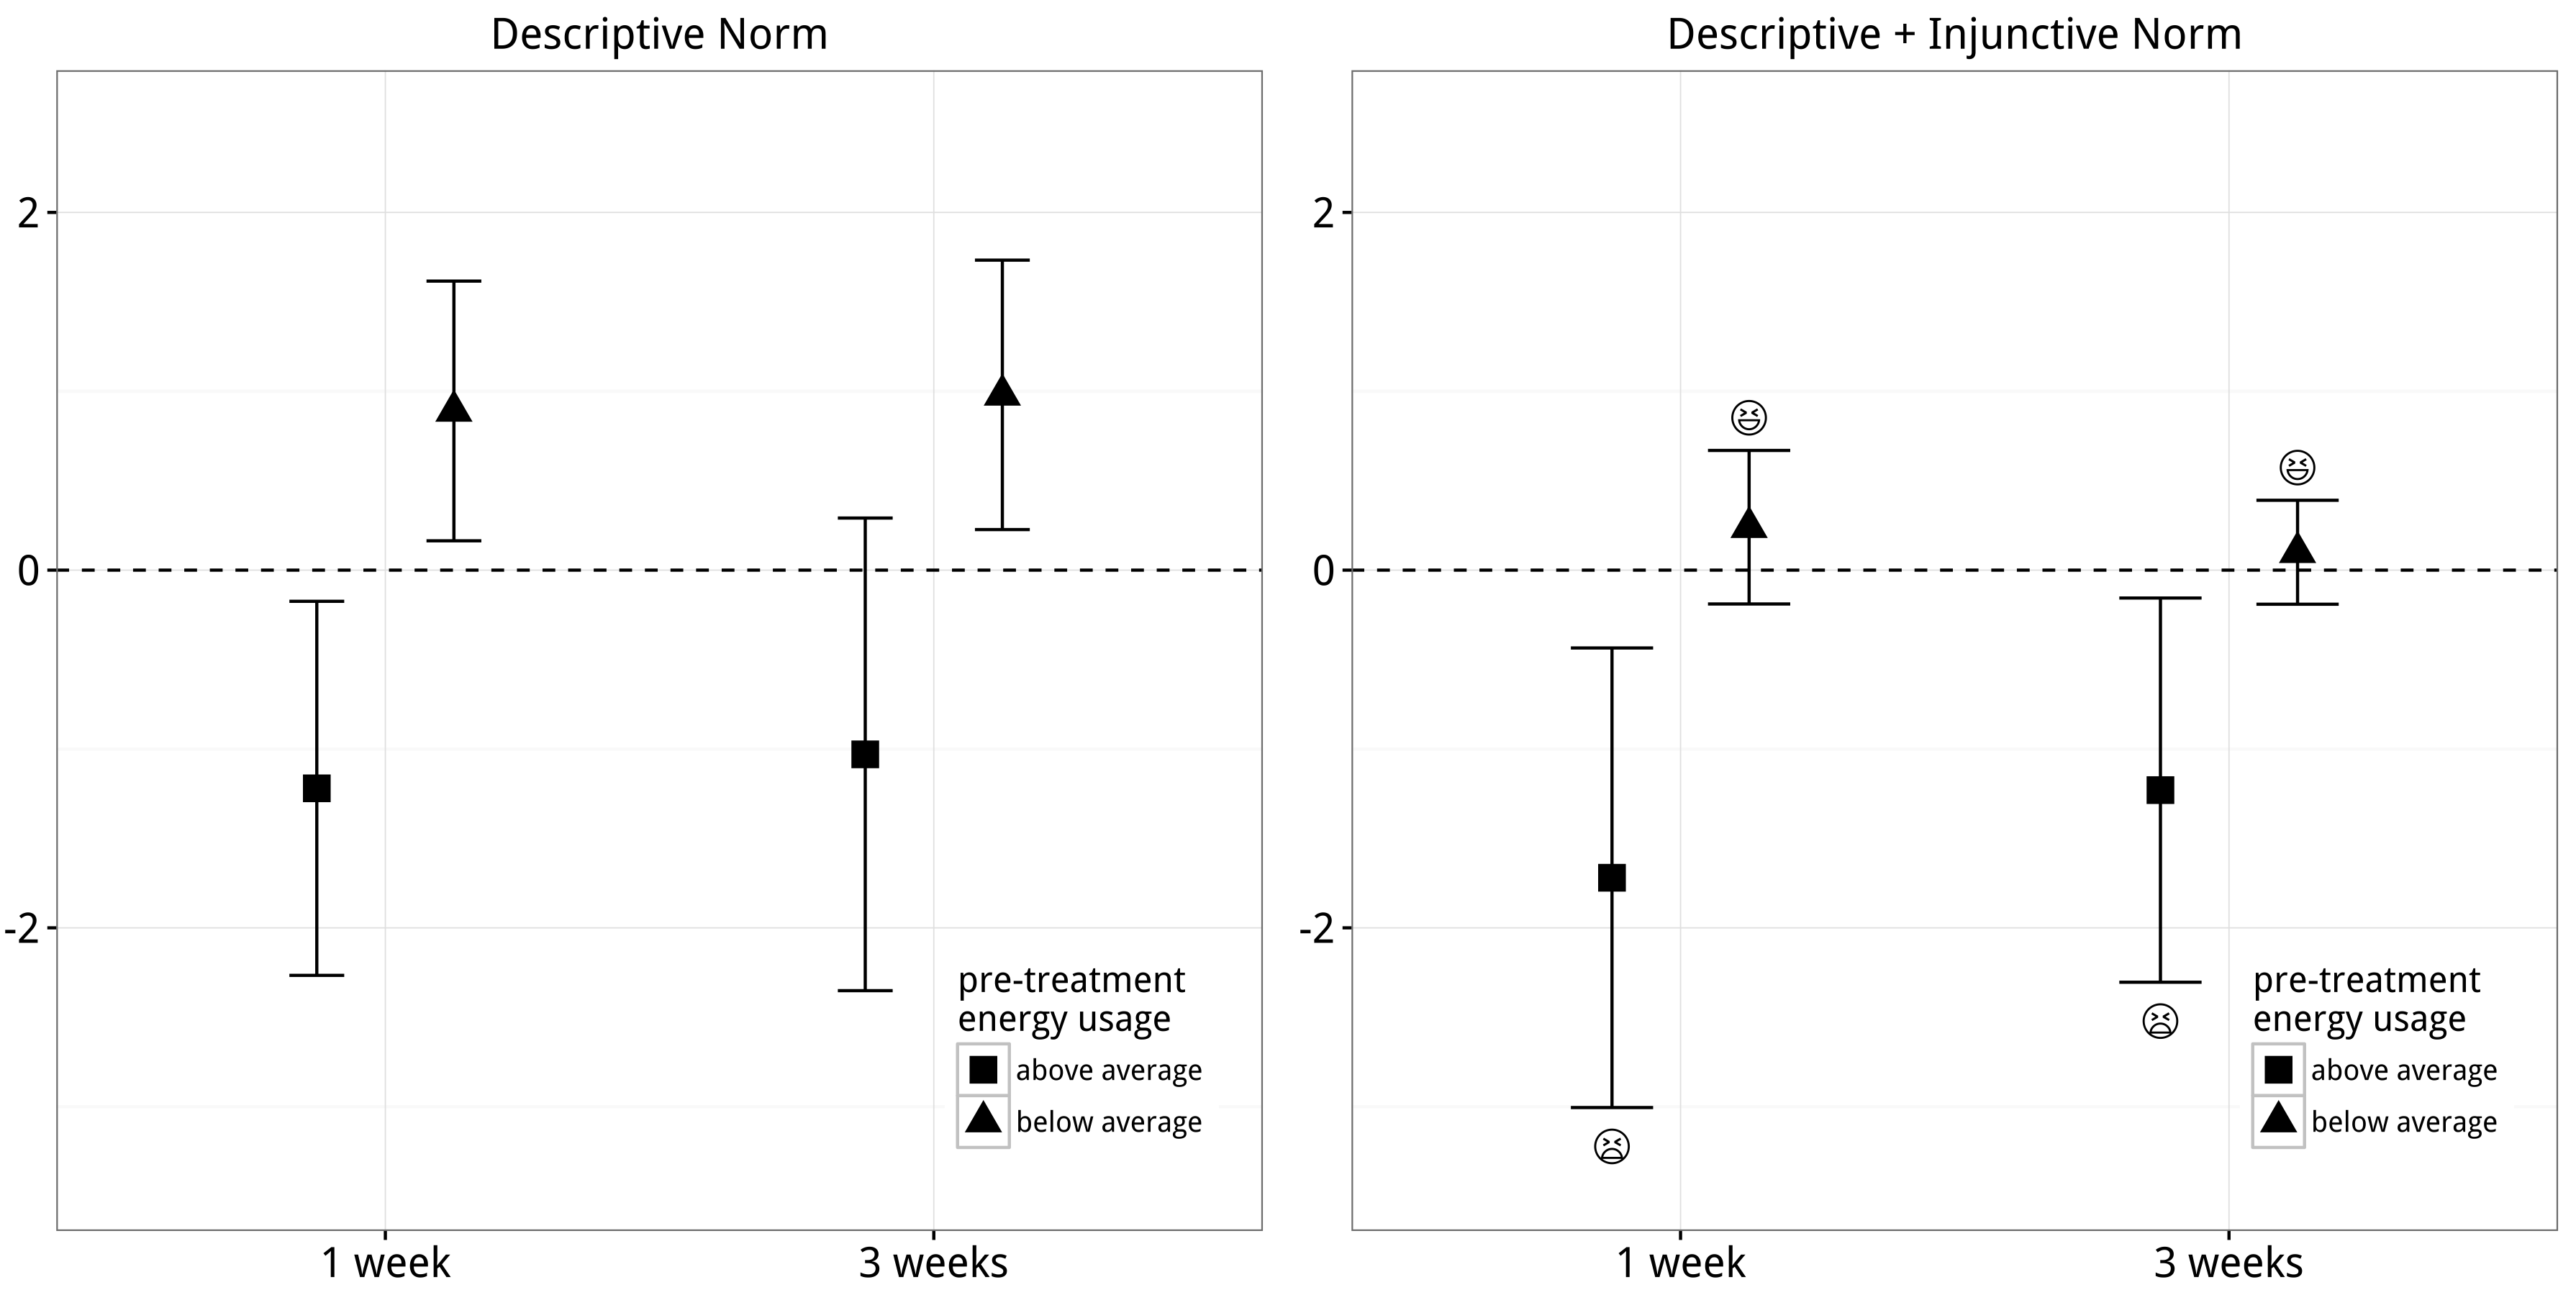
\includegraphics[width = \textwidth]{figures/schultz_constructive_2007_23panel}
\end{figure}

\end{frame}
%%%%%%%%%%%%%%%%%%%%%%%%
\begin{frame}

If you want to move beyond simple experiments:
\begin{itemize}
\item Validity
\item Heterogeneity of treatment effects
\item Mechanisms
\end{itemize}

\end{frame}
%%%%%%%%%%%%%%%%%%%%%%%%%%%
\begin{frame}

Validity
\begin{itemize}
\item statistical conclusion validity
\item internal validity
\item construct validity
\item external validity
\end{itemize}

\end{frame}
%%%%%%%%%%%%%%%%%%%%%%%%%%%
\begin{frame}

Heterogeneous treatment effects 
\begin{itemize}
\item lots of people, lots of pre-treatment information: stop treating people like widgets
\pause
\item beware of fishing
\pause
\item Lots of new methods in this area
\end{itemize}

\end{frame}
%%%%%%%%%%%%%%%%%%%%%%%%%%%
\begin{frame}

Mechanisms
\begin{itemize}
\item Not as easy as scurry and limes, ``Enough already about black box experiments''  \textcolor{blue}{\href{http://dx.doi.org/10.1177/0002716209351526}{Green et al (2010)}}
\pause
\item Experiments specifically designed to test mechanisms: \textcolor{blue}{\href{http://dx.doi.org/10.1257/jep.25.3.17}{Ludwig et al (2011)}}, \textcolor{blue}{\href{http://dx.doi.org/10.1111/j.1467-985X.2012.01032.x}{Imai et al (2012)}}, \textcolor{blue}{\href{http://dx.doi.org/10.1016/j.jesp.2015.09.012}{Pirlott and MacKinnon (2016)}}
\end{itemize}

\end{frame}
%%%%%%%%%%%%%%%%%%%%%%%%%%%
\begin{frame}

\Large{
\begin{center}
Optimization experiments + Understanding experiments
\end{center}
}

\pause
This is particularly important if you want to partner with the powerful.  But it is very hard.

\end{frame}
%%%%%%%%%%%%%%%%%%%%%%%
\begin{frame}

\Large{
\begin{center}
Questions?
\end{center}
}

\end{frame}
%%%%%%%%%%%%%%%%%%%%%%%




\end{document}
